
\section*{Results}

The results of the calculations performed by the two Python scripts are summarized in the following tables. The first script analyzed the overall average number of pions produced by the collisions for each events and their difference.
The second script calculated the number of positive and negative pions in function of pseudorapidity and transverse momentum, as well as the differences between pions and anti-pions.
\\

Table 1 presents the results for the average number per event of both positive and negative pions produced by the collisions. The mean difference between positive and negative pions is also displayed.
7,5
\begin{table}[ht]
    \centering
    \caption{Average Amount of Positive and Negative Pions}
    \begin{tabular}{|l|c|c|}
        \hline
        Pion Type                      & {Average Amount}       & {Uncertainty}         \\ \hline
        Positive Pions                 & 18.43                & ± 0.03             \\ \hline
        Negative Pions                 & 18.40                & ± 0.03              \\ \hline
        Difference of Means            & 0.030                 & ± 0.004            \\ \hline
    \end{tabular}
\end{table}
\newpage
Graphs (a) and (b) display the number of pions (in blue) and anti-pions (in orange) per event, along with their corresponding uncertainties, as a function of pseudorapidity and transverse momentum ranges, respectively.

\begin{figure}[H]
  \centering
  % First row with Figures 1 and 2
  \begin{subfigure}{0.49\textwidth}
    \centering
    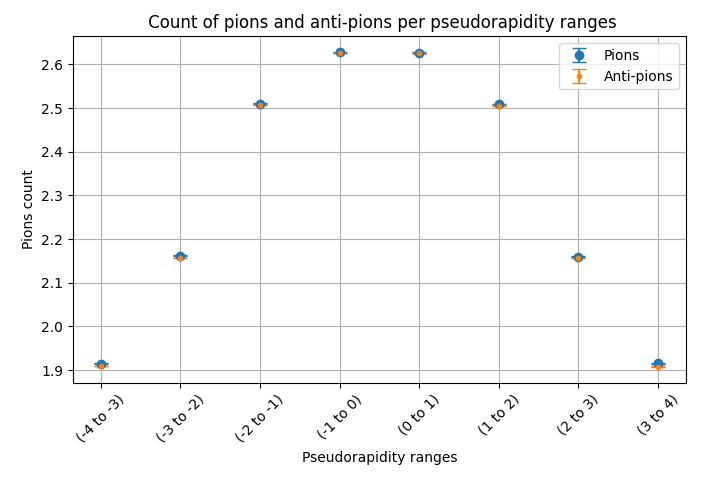
\includegraphics[width=\linewidth]{lab report/Figure_1_final.png}
    \caption{Count of pions as a function of pseudorapidity}
    \label{fig:subfig1}
  \end{subfigure}
  \hfill
  \begin{subfigure}{0.49\textwidth}
    \centering
    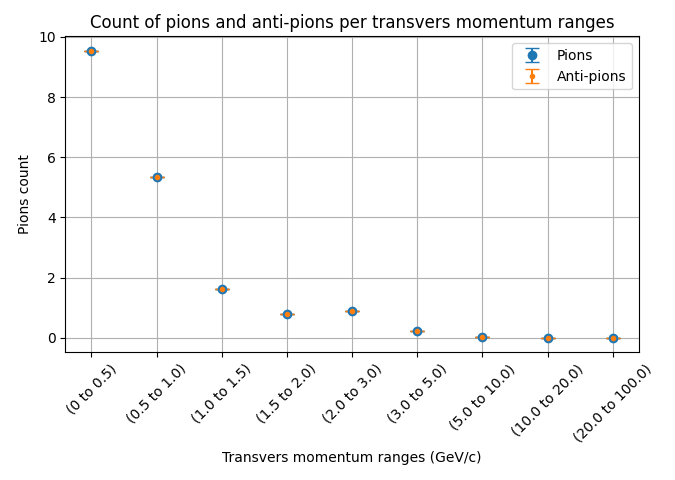
\includegraphics[width=\linewidth]{lab report/Figure_2_final.png}
    \caption{Count of pions as a function of transverse momentum}
    \label{fig:subfig2}
  \end{subfigure}
  
  \vskip\baselineskip  % Adds vertical space between rows
  
  % Second row with Figures 3 and 4
  \begin{subfigure}{0.49\textwidth}
    \centering
    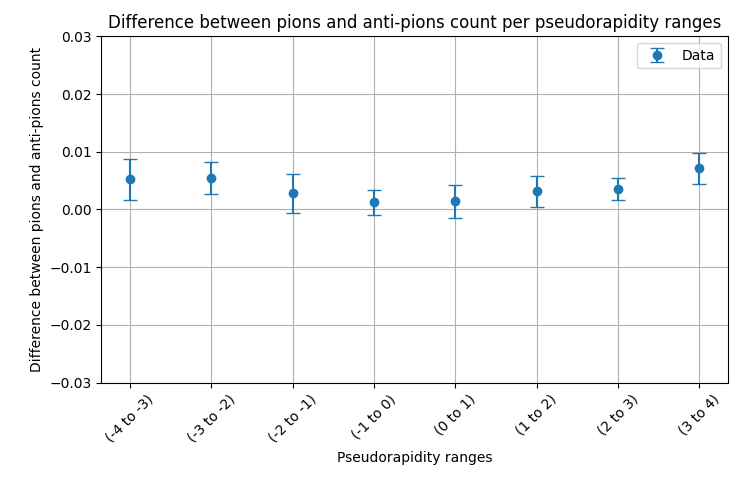
\includegraphics[width=\linewidth]{lab report/Figure_3_final.png}
    \caption{Difference in pion count as a function of pseudorapidity}
    \label{fig:subfig3}
  \end{subfigure}
  \hfill
  \begin{subfigure}{0.49\textwidth}
    \centering
    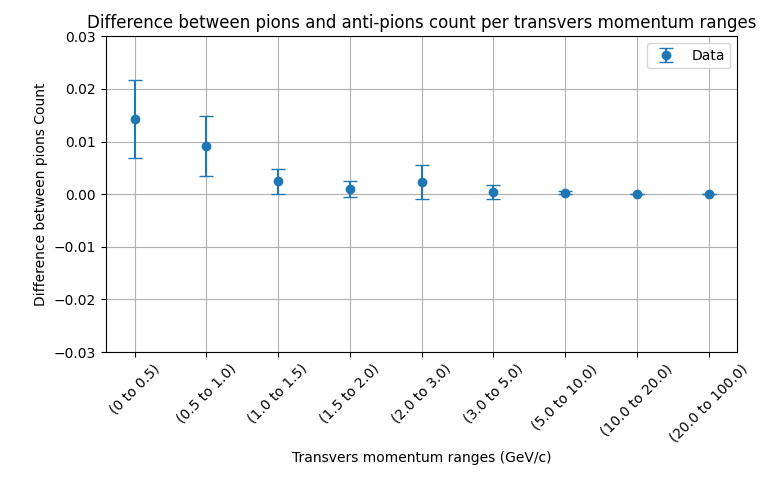
\includegraphics[width=\linewidth]{lab report/Figure_4_final.png}
    \caption{Difference in pion count as a function of transverse momentum}
    \label{fig:subfig4}
  \end{subfigure}
\end{figure}
